\section{Adaptive Learning Algorithms}

\begin{frame}
\frametitle{Agenda}
\tableofcontents[currentsection]
\end{frame}


% --------------------------------------------------------------------------------------------------------------
\begin{frame}
\frametitle{Adaptive Learning Algorithms}

\begin{de}{Adaptive Learning Algorithm}
can be seen as advanced incremental learning
algorithms that are able to adapt to evolution of the data-generating process over time.
\end{de}

It needs to be able to:
\begin{enumerate}

\item detect concept drift (and adapt if needed) as soon as possible;

\item distinguish drifts from noise and be adaptive to changes, but robust to noise; and

\item operate in less than example arrival time and use not more than a fixed amount of
memory for any storage.
\end{enumerate}


\end{frame}
% --------------------------------------------------------------------------------------------------------------

\begin{frame}
\frametitle{Online Adaptive Learning Procedure}

\begin{figure}
	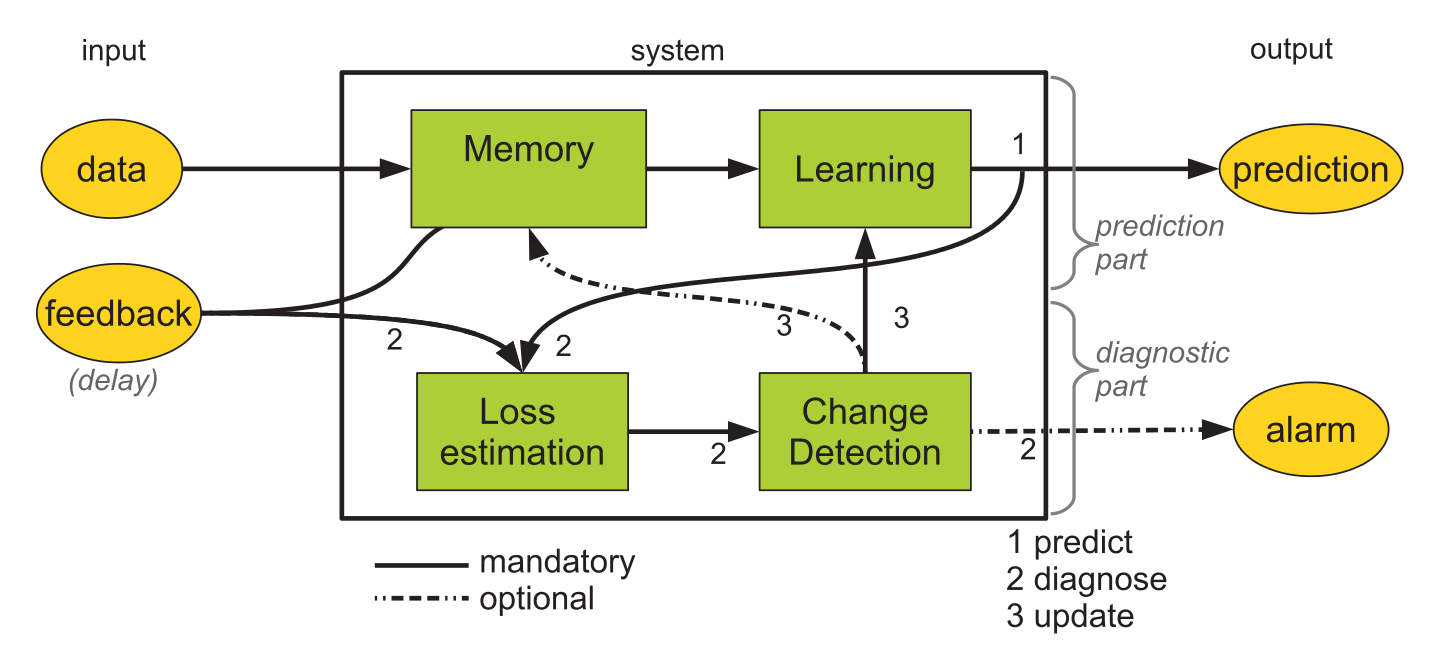
\includegraphics[width=0.75\textwidth]{modelala}
\end{figure}

\begin{enumerate}
	\item \textit{Predict.} When new example $X_t$ arrives, a prediction $\hat{y_t}$ is made using the curren model $L_t$.
	\item<2-3> \textit{Diagnose.} After some time, the true label $y_t$ is received and we can estimate the loss as $f(\hat{y_t}, y_t)$.
	\item<3> \textit{Update.} We can use the example $(X_t,y_t)$ for the model update to obtain $L_{t+1}$.
\end{enumerate}

\end{frame}


% --------------------------------------------------------------------------------------------------------------
\begin{frame}[allowframebreaks]
\frametitle{Concept drift}
\begin{de}{Concept drift}
Formally, concept drift between time point $t_0$ and time point $t_1$ can be defined as:
$$\exists X:p_{t_0}(X,y) \neq p_{t_1}(X,y)$$

where $p_{t_0}$ denotes the joint distribution at time $t_0$ between the set of input variables X and the target variable y.
\end{de}


%Changes in data:

%\begin{itemize}
%\item prior probablities of classes $p(y)$ may change.
%\item class conditional probabilites $p(X|y)$ may change
%\item as a result the posterior probablities of classes $p(y|X)$ may change %(afftects the prediciton).
%\end{itemize}

\framebreak
$$\exists X:p_{t_0}(X,y) \neq p_{t_1}(X,y)$$
\begin{de}{Real concept drift}
refers to changes in $p(y|X)$. Such changes can happen either with
or without change in $p(X)$. It's also called \textit{concept shift} or \textit{conditional change}.
\end{de}

\begin{de}{Virtual concept drift}
happens if the distribution of the incoming data chagnes (i.e., p(X) changes) without affecting $p(y|X)$.
\end{de}
\end{frame}
% --------------------------------------------------------------------------------------------------------------


% --------------------------------------------------------------------------------------------------------------
\begin{frame}
\frametitle{Example: real vs. virtual drift}
\begin{figure}
	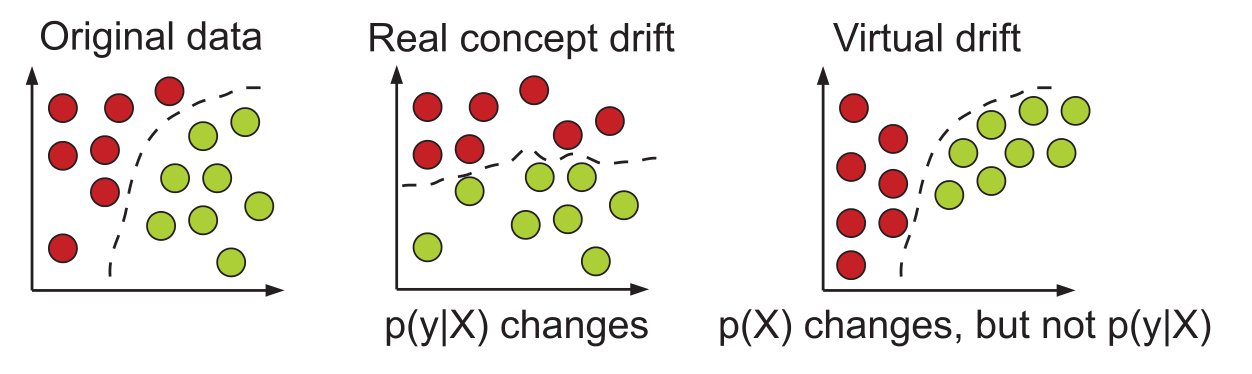
\includegraphics[width=\textwidth]{types}
\end{figure}
\textit{Circles} represent instances.\\
Different \textit{colors} represent different classes.

\end{frame}
% --------------------------------------------------------------------------------------------------------------

% --------------------------------------------------------------------------------------------------------------
\begin{frame}
\frametitle{A practical example: \# of people in a library}
\begin{figure}
	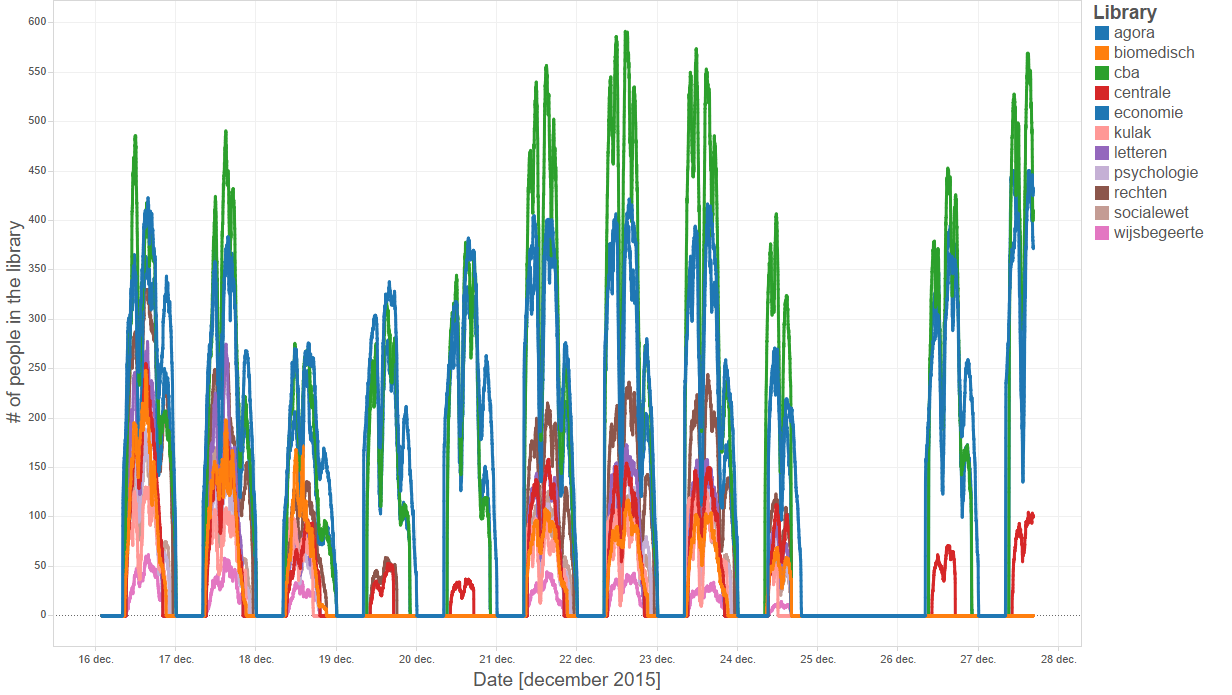
\includegraphics[width=\textwidth]{general_all}
	\caption	{\# of people in the KU Leuven libraries}
\end{figure}

\end{frame}

\begin{frame}
\frametitle{A practical example: \# of people in a library}
\begin{figure}
	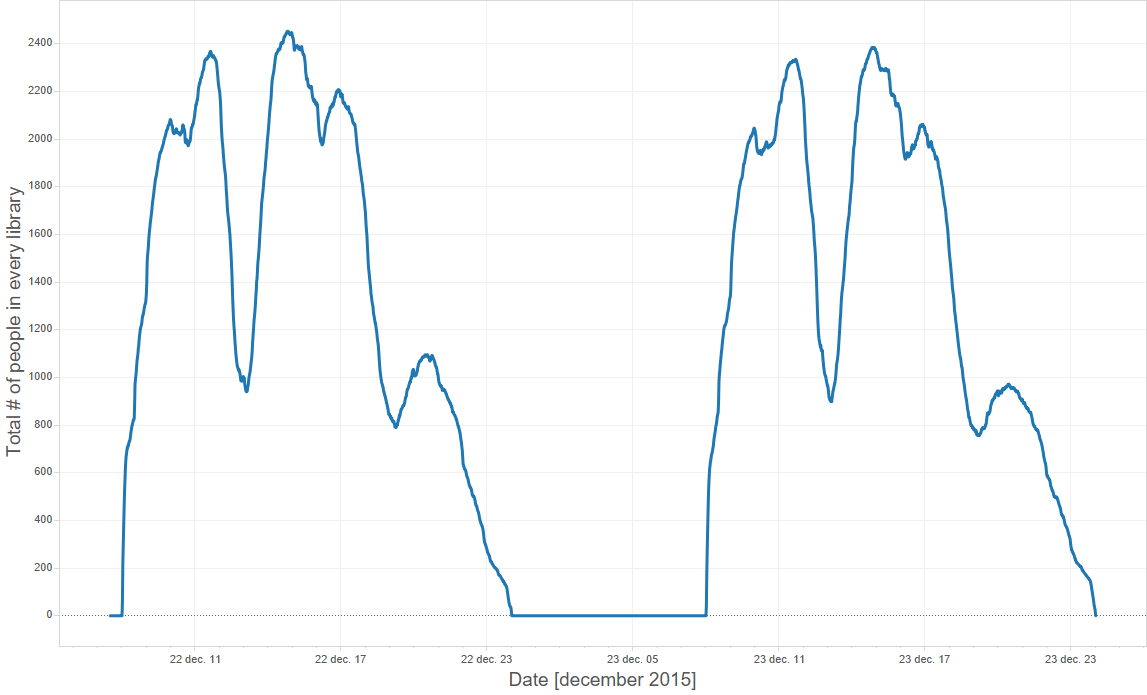
\includegraphics[width=0.75\textwidth]{total}
	\caption	{Sum of people in all KU Leuven libraries}
\end{figure}
\textbf{Task:} predict the total amount of people in all libraries\\
If same amount of people go to different libraries: \only<2>{$\rightarrow$ virtual drift}
\end{frame}
% --------------------------------------------------------------------------------------------------------------
\begin{frame}
\frametitle{A practical example: \# of people in a library}
\begin{figure}
	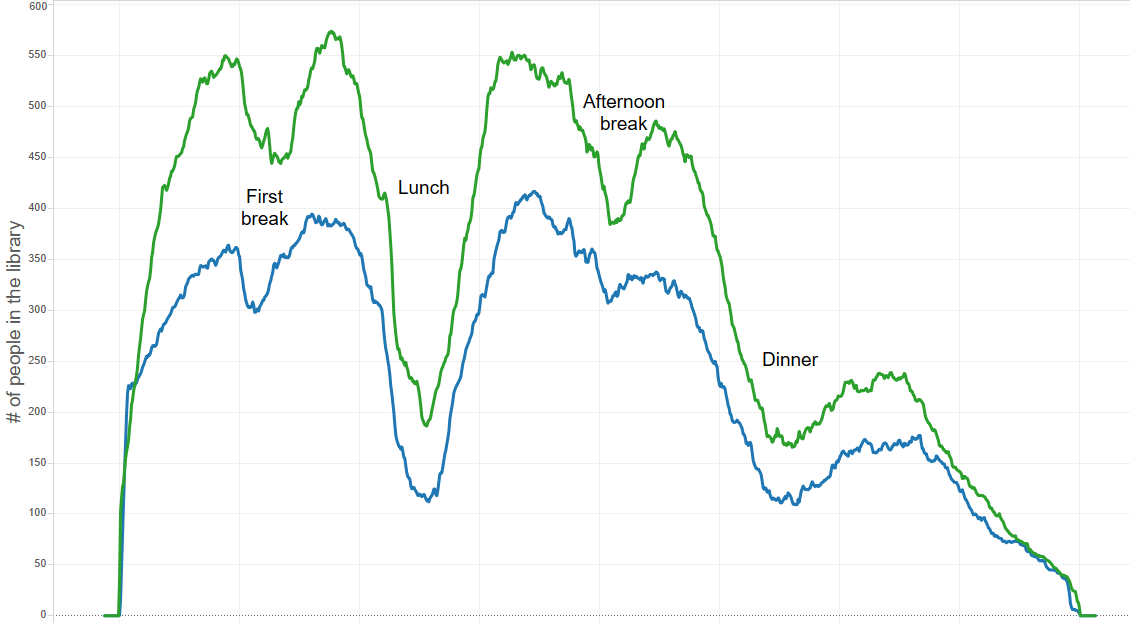
\includegraphics[width=0.75\textwidth]{comparison}
	\caption	{Sum of people in all KU Leuven libraries}
\end{figure}
\textbf{Task:} predict percentage of people in a specific library on a monday\\
If some people go to different libraries: \only<2>{$\rightarrow$ real drift}
\end{frame}

\begin{frame}
\frametitle{Changes in drift over time}

\begin{figure}[H]

	\begin{subfigure}[H]{0.2\textwidth}
		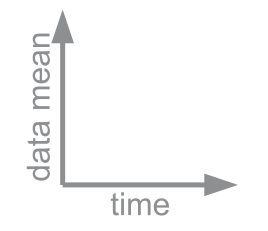
\includegraphics[width=\textwidth]{cot0}
	\end{subfigure}
	~
	\begin{subfigure}[H]{0.4\textwidth}
		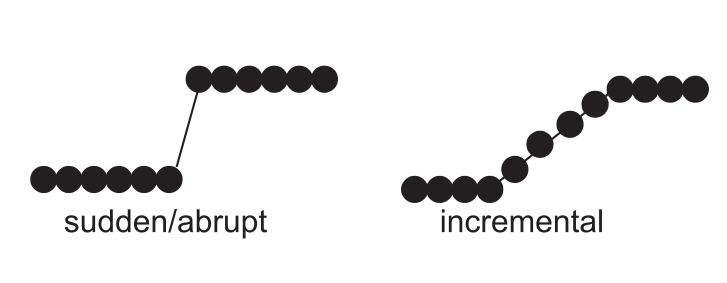
\includegraphics[width=\textwidth]{cot1}
	\end{subfigure}
	
	\only<2>{
	\begin{subfigure}[H]{0.2\textwidth}
		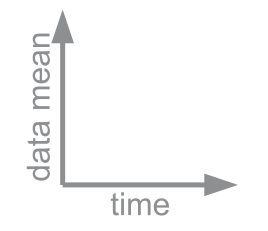
\includegraphics[width=\textwidth]{cot0}
	\end{subfigure}
	~
	\begin{subfigure}[H]{0.4\textwidth}
		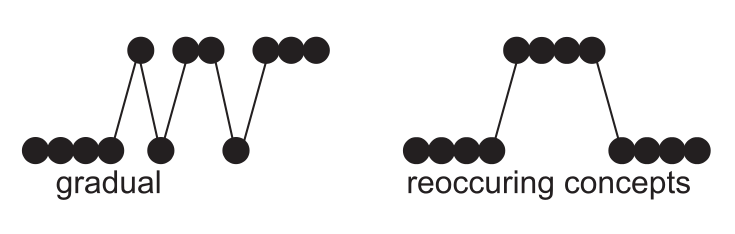
\includegraphics[width=\textwidth]{cot2}
	\end{subfigure}}
	
	\only<3>{
	\begin{subfigure}[H]{0.2\textwidth}
		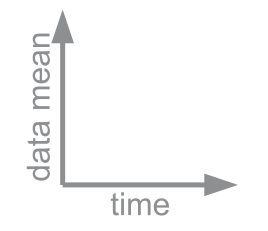
\includegraphics[width=\textwidth]{cot0}
	\end{subfigure}
	~
	\begin{subfigure}[H]{0.4\textwidth}
		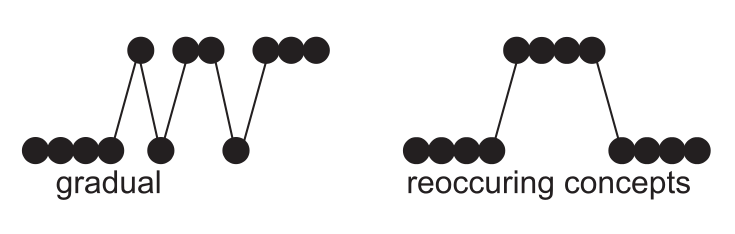
\includegraphics[width=\textwidth]{cot2}
	\end{subfigure}
	
	\begin{subfigure}[H]{0.2\textwidth}
		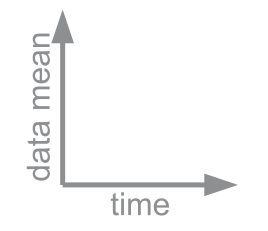
\includegraphics[width=\textwidth]{cot0}
	\end{subfigure}
	~
	\begin{subfigure}[H]{0.25\textwidth}
		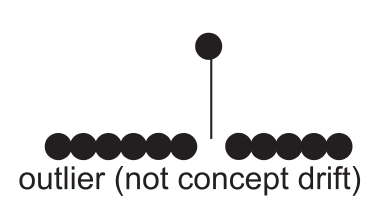
\includegraphics[width=\textwidth]{cot3}
	\end{subfigure}}
\end{figure}

\end{frame}


\begin{frame}
\frametitle{Changes in drift over time: library example}

\begin{figure}[H]
	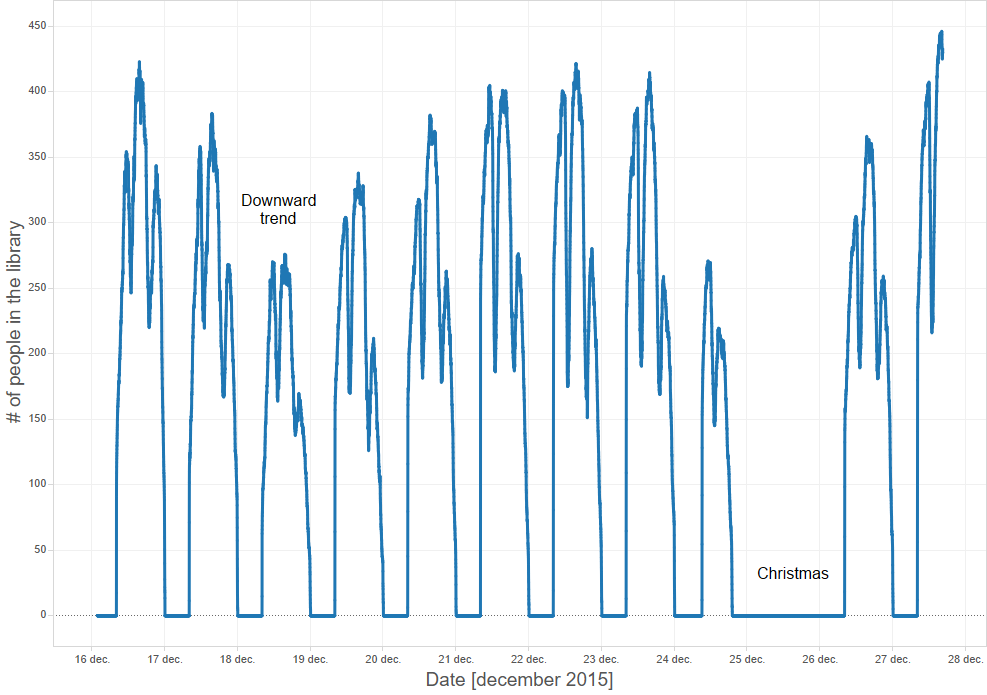
\includegraphics[width=\textwidth]{general}
\end{figure}
\end{frame}


\begin{frame}
\frametitle{Illustrative Applications}
\begin{itemize}
	
	\item Management and strategic planning
	\only<1>{
		\begin{figure}[H]
			\centering
			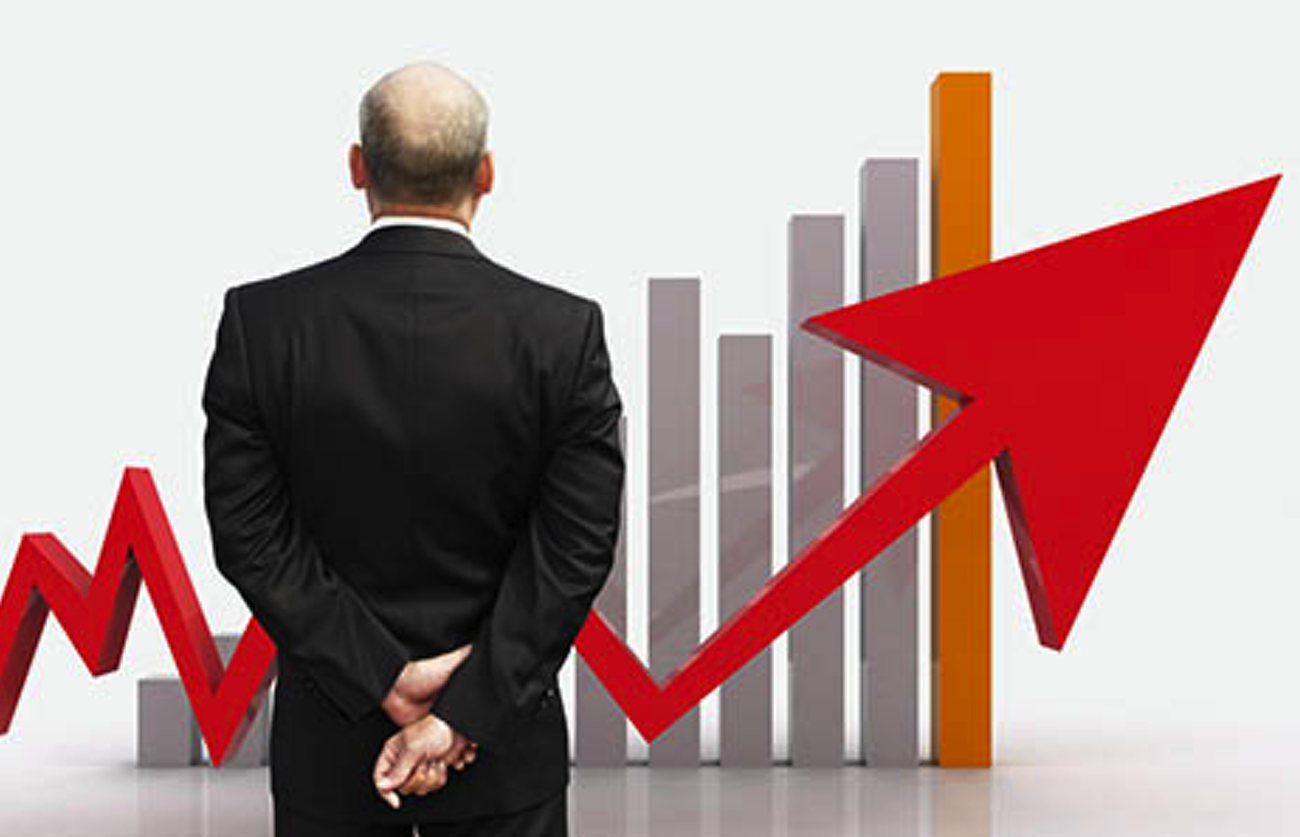
\includegraphics[width=0.75\textwidth]{forecast}
		\end{figure}
	}
	
	\item Personal assistance and information
	\only<2>{
		\begin{figure}[H]
			\centering
			
\includegraphics[width=0.75\textwidth]{netflix}
		\end{figure}
	}
	
	\item Ubiquitous environment applications
	\only<3>{
		\begin{figure}[H]
			\centering
			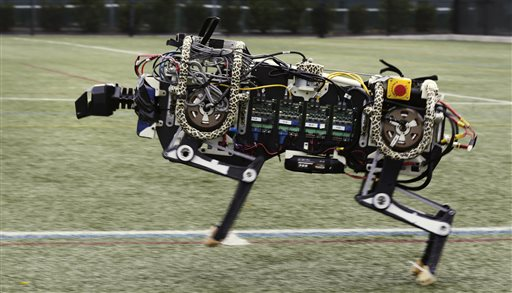
\includegraphics[width=0.75\textwidth]{cheetah}
		\end{figure}
	}
\end{itemize}
\end{frame}

